
\newpage

\thispagestyle{empty}
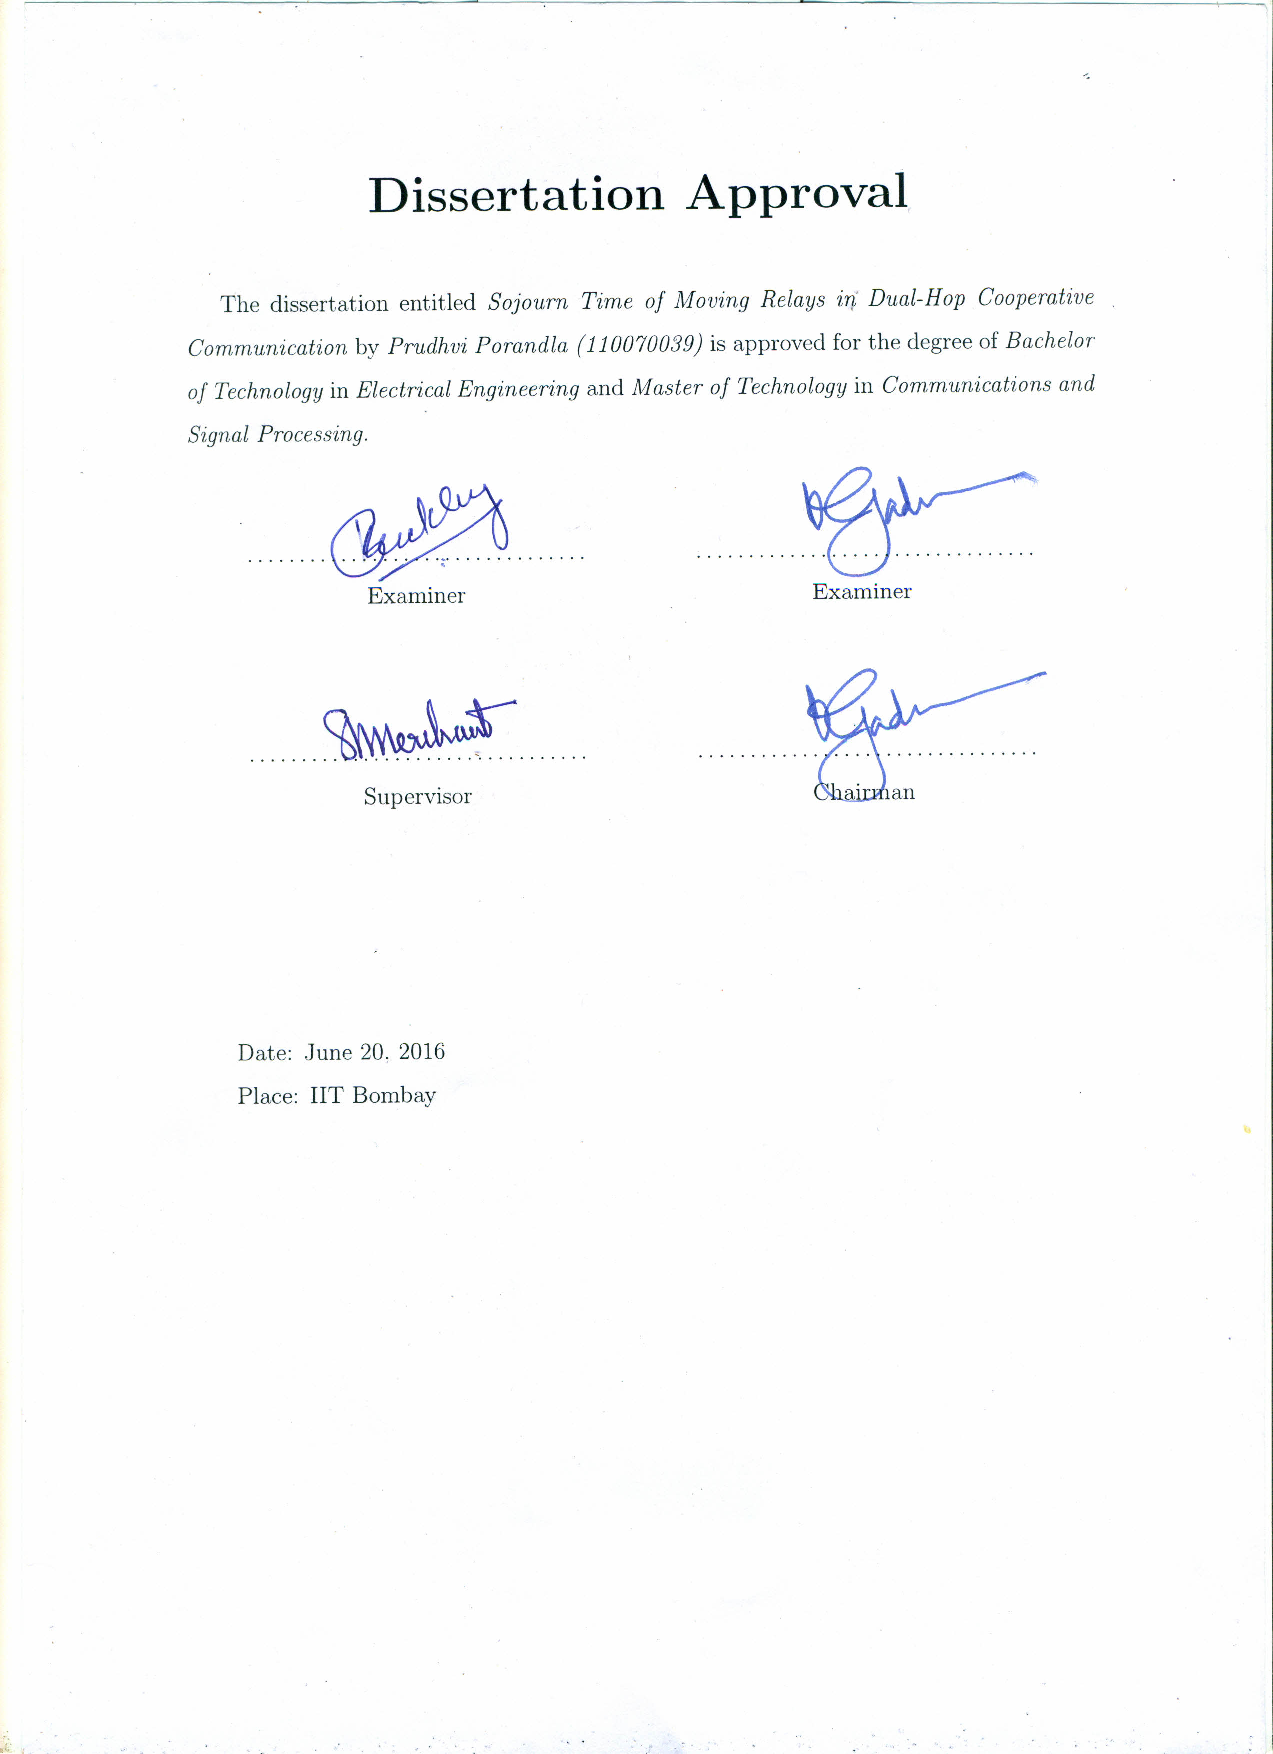
\includepdf{approval.pdf}
\begin{comment}
\begin{center}
  \begin{Huge}
    \textsc{\textbf{Dissertation Approval}}
  \end{Huge}
\end{center}

\vspace{0.2in}

 The dissertation entitled \textit{Sojourn Time of Moving Relays in Dual-Hop Cooperative Communication} by \textit{Prudhvi Porandla (110070039)} is approved for the degree of \textit{Bachelor of Technology} in \textit{Electrical Engineering} and \textit{Master of Technology} in \textit{Communications and Signal Processing.}


\vspace{0.1in}
%\begin{flushright}
%\textbf{Examiners} \\
%\vspace{1.5in}
%\textbf{Supervisors}\\
%\vspace{1.5in}
% \textbf{Chairman}\\

%\end{flushright}
%\vspace{0.7in}
%Date :    \\
%Place :\\
%\begin{table*}[hb]
%\begin{center}
%\begin{tabular}{ll}
%\textbf{Prof.  IITB} & \hspace{0.7in} \textbf{Prof. , IITB}\\
%(Internal Examiner) & \hspace{0.7in} (External Examiner)\\
%\vspace{0.5in}\\
%\textbf{Prof. Rajbabu Velmurugan, IITB} & \hspace{0.7in}  \textbf{Prof. Sibiraj Pillai, IITB} \\ 
%(Guide) & \hspace{0.7in} (Co-Guide)\\
%\vspace{0.5in}\\
%\textbf{Prof. , IITB}\\
%(Chairman)\\
%\end{tabular} \vspace{0.2in}
%\end{center}
%\begin{tabular}{ll}
%Date: & May 22, 2015 \\ \vspace{30pt}
%Place: & Indian Institute of Technology Bombay, Mumbai\\
%\end{tabular}
%
%\end{table*}
\begin{center}
	\begin{tabular}{ccc}
		\rule{60mm}{0pt}        & \rule{10mm}{0pt}       & \rule{60mm}{0pt} \\
		\dotfill                &                        & \dotfill \\
		Examiner                &					     & Examiner \vspace{2cm} \\
		\dotfill                &                        & \dotfill \\
		Supervisor              &                        & Chairman \vspace{2cm} \\
	\end{tabular}    
\end{center}

\vspace{5mm}
\begin{tabular}{lll}
	\rule{40mm}{0pt}        & \rule{50mm}{0pt}       & \rule{60mm}{0pt} \\
	Date: June 20, 2016		&                        & \\
	Place: IIT Bombay       &                        & \\
\end{tabular}
%\newpage
%\thispagestyle{empty}
%\mbox{}
%  \newpage
\end{comment}
\newpage
\thispagestyle{empty}
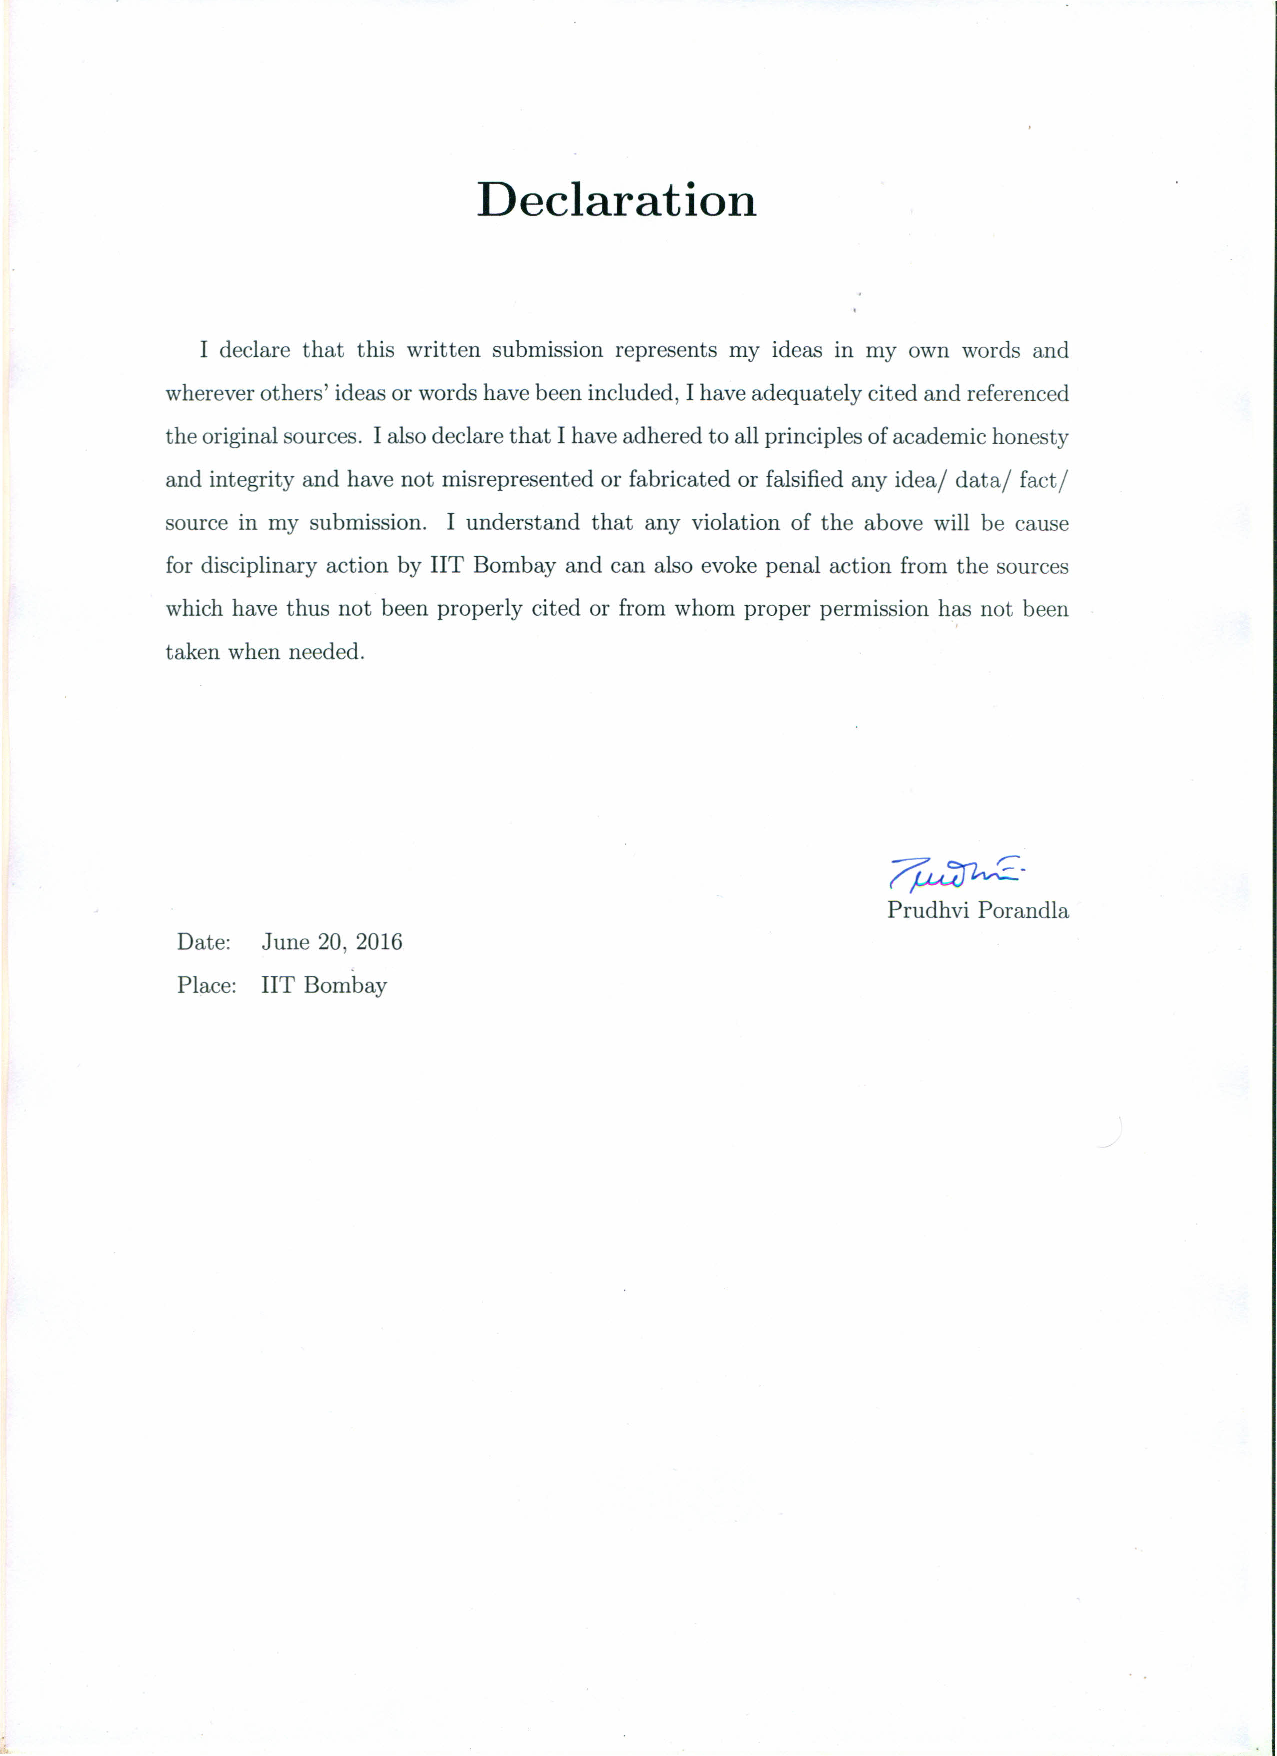
\includepdf{signedDeclaration.pdf}

\begin{comment}
\begin{center}
	\begin{Huge}
		\textsc{\textbf{Declaration}}
	\end{Huge}
\end{center}

\vspace{0.5in}

 I declare that this written submission represents my ideas in my own words and wherever others' ideas or words have been included, I have adequately cited and referenced the original sources. I also declare that I have adhered to all principles of academic honesty and integrity and have not misrepresented or fabricated or falsified any idea/ data/ fact/ source in my submission. I understand that any violation of the above will be cause for disciplinary action by IIT Bombay and can also evoke penal action from the sources which have thus not been properly cited or from whom proper permission has not been taken when needed.

\vspace{1.5in}
% \begin{table*}[hb]
% \begin{center}
	\hfill Prudhvi Porandla\\
	\noindent
	\begin{tabular}{ll}
		Date: & June 20, 2016\\ \vspace{30pt}
		Place: & IIT Bombay\\
	\end{tabular}
	% 

	% \begin{dedication}
		\newpage
		\thispagestyle{empty}    % No page number

	%	\begin{center}  \null\vfill
	%		\textit{\Large To YOU}
	%		\null\vfill
	%	\end{center}
		% \newpage

		% \end{dedication}
		%\newpage
		%\thispagestyle{empty}
		%\mbox{}
\end{comment}




	\newpage
	\thispagestyle{empty}
	\begin{center}
		\begin{Huge}
			\textsc{\textbf{Acknowledgements}}
		\end{Huge}
	\end{center}

	\vspace{0.25in}

	I would to express my heartfelt gratitude to my guide Prof. S. N. Merchant for his constant encouragement and patience throughout the project. I would like to thank him for offering moral support to work on the project by placing overwhelming amount of trust in me.    

	I would like to thank Kesav Kaza for his support, advice and presence during every technical discussion and brainstorming session. This work is essentially the summation of all the ideas exchanged during those sessions. I would like to thank all SPANN lab members for making every moment in the lab a learning experience. Special thanks to Zoheb for providing some of the figures. Finally, my wholehearted thanks to the faculty members of Electrical Engineering Department for imparting me with invaluable knowledge. 

	I owe my deepest gratitude to my parents for their relentless support throughout my life and their patience during my DDP work. To the power that drives the Nature without which nothing is possible. 


	\vspace{0.6in}
	\noindent June 20, 2016    \hfill Prudhvi Porandla\\


	%\newpage
	%\thispagestyle{empty}
	%\mbox{}


	\clearpage\pagenumbering{roman} 
	\begin{abstract}

		We explore the application of relaying in cellular networks and study various cooperation policies. We propose a cooperation policy for downlink using the same principles that were used to design policies in uplink case. We then discuss the case where relays are moving according to a random waypoint(RWP) mobility model. We attempt to find the sojourn time of a relay in the feasible region and present the challenges involved. As a first advance towards finding the sojourn time we give a general expression for the probability that a relay leaves the feasible region in one step that can be used for any mobility model. We use the probability to find the expected number of transitions a node makes before leaving the region and compare it with the simulation results. Finally we present the idea of modelling the node movement as a Markov Chain and to use the results of Absorbing Markov Chain to find the expected number of transitions more accurately. 

	\end{abstract}
	\newpage
	\mbox{}
	\newpage
